\documentclass{beamer}
\usepackage{amsmath} 
\usepackage{graphicx} 
\usepackage{color}
\usepackage[utf8]{inputenc}
\usepackage{subfigure}
\usepackage{caption}
\usepackage{bm}
%\captionsetup{font={scriptsize}}
\title{Monte Carlo Simulation of Two-dimensional Ising model}
\author{Tong Li}
\institute{Department of Physics \& Astronomy \\ Michigan State University }
\date{\today}
\setbeamertemplate{footline}[frame number] 
\usecolortheme{seahorse}
\setbeamertemplate{caption}[numbered]

\makeatletter
\def\blfootnote{\gdef\@thefnmark{}\@footnotetext}
\makeatother

\renewcommand{\thefootnote}{\fnsymbol{footnote}}

\begin{document}
\beamertemplatenavigationsymbolsempty

\thispagestyle{empty} 
\begin{frame}
\titlepage
\end{frame}

\begin{frame}{Outline}
\tableofcontents
\end{frame} 

\section{Introduction}	
\begin{frame}{Introduction}
\begin{itemize}
	\item <1-> Ising model is a simple but important model for the explanation of ferromagnetism.  
	\item <2-> Assumption 1: \\
	Atomic spins are located on a $N$-dimensional lattice grid, 
	and these spins only have two discrete states, up ($\sigma=1$) or down ($\sigma=-1$). 
	\item <3-> Assumption 2: \\
	Only neighboring spins can interact with each other, and thus its Hamiltonian can be written as 
	\begin{equation}\label{eq:hamiltonian}
	H=-J\sum_{<kl>}^{N}\sigma_k\sigma_l\,, 
	\end{equation}
	where $J>0$ and $<kl>$ indicates that we only sum over nearest neighbors. 
\end{itemize}
\end{frame}

\begin{frame}{Introduction}
\begin{itemize}
	\item <1-> Only one- and two-dimensional cases has been solved analytically and they show several interesting properties of phase transition. 
	\item <1-> Therefore, it is necessary to develop a numerical method for the simulation of Ising model. 
	\item <2-> In this work we focus on the Monte Carlo simulation of 2D Ising model, which can be benchmarked with analytical solution. 
	\item <3-> Our numerical framework can also be easily extended to higher dimensions. 
\end{itemize}
\end{frame}

\section{Properties of 2D Ising model from its analytical solution}

\begin{frame}{Outline}
\tableofcontents[currentsection]
\end{frame}

\subsection{The solution of $2 \times 2$ Ising model}
\begin{frame}{Properties of 2D Ising model from its analytical solution}
To be filled. 
\end{frame}

\subsection{Properties of phase transition in 2D Ising model}
\begin{frame}{Properties of phase transition in 2D Ising model}
To be filled. 
\end{frame}

\section{Monte Carlo methods for Ising model}
\begin{frame}{Outline}
\tableofcontents[currentsection]
\end{frame}

\begin{frame}{Monte Carlo methods for Ising model}
To be filled. 
\end{frame}

\section{Results and discussion}
\begin{frame}{Outline}
\tableofcontents[currentsection]
\end{frame}

\subsection{Results of $2 \times 2$ case}
\begin{frame}{Results of $2 \times 2$ case}
\begin{table}
	\centering
	\caption{Results for $2\times2$ case with temperature $T=1.0$. Analytical results are provided for benchmark. 
		Energy is in the unit of $J$. }
	\begin{tabular}{cccccc}
		\hline
		\hline
		$MC$ & 10 & 100 & 1000 & 10000 & Analytical \\ 
		\hline
		$\langle E \rangle$ & -7.2 & -7.92 & -7.986 & -7.988 & -7.98393\\ 
		$\langle |M| \rangle$ & 3.75 & 3.975 & 3.9955 & 3.99625 & 3.99263\\ 
		$\langle E^2 \rangle$ & 57.6  & 63.36 & 63.888 & 63.904 & 63.8714\\ 
		$\langle M^2 \rangle$ & 14.7 & 15.87 & 15.977 & 15.9805 & 15.9732\\ 
		$C_V$ & 5.76 & 0.6336 & 0.111804 & 0.095856 & 0.128329\\ 
		$\chi$ & 0.6375 & 0.069375 & 0.0129798 & 0.0104859 & 0.0320873\\ 
		\hline
		\hline 
	\end{tabular} 
	\label{tab:2times2result}
\end{table}
\end{frame}

\subsection{Convergence and probability distribution}
\begin{frame}{Convergence and probability distribution}
\begin{figure}
	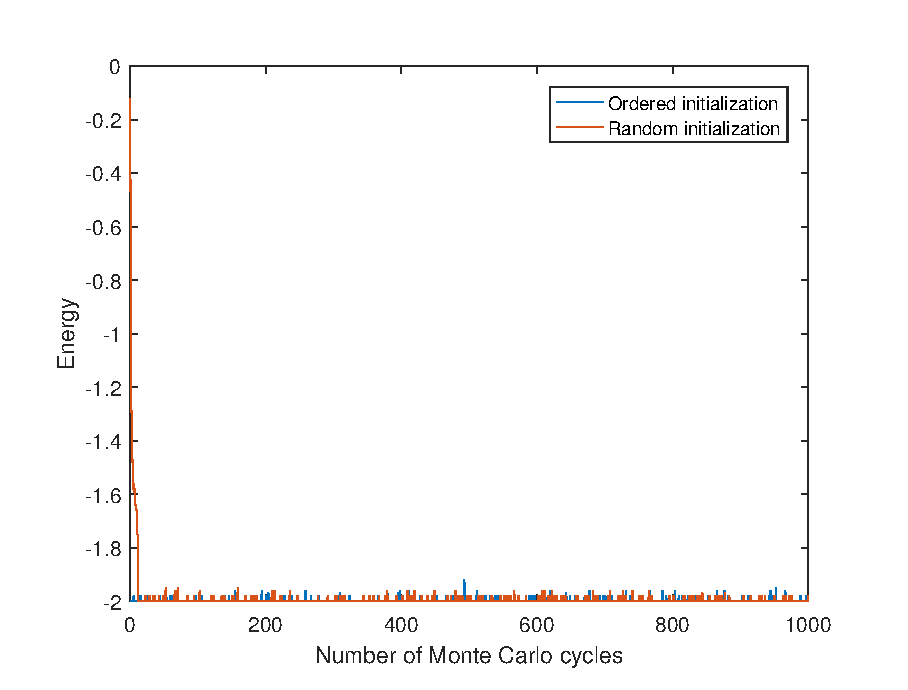
\includegraphics[width=0.8\textwidth]{Process_ene_lowT.eps}
	\caption{Energy as a function of the number of Monte Carlo cycles for $T=1.0$, $L=20$. }
\end{figure}
\end{frame}

\begin{frame}{Convergence and probability distribution}
\begin{figure}
	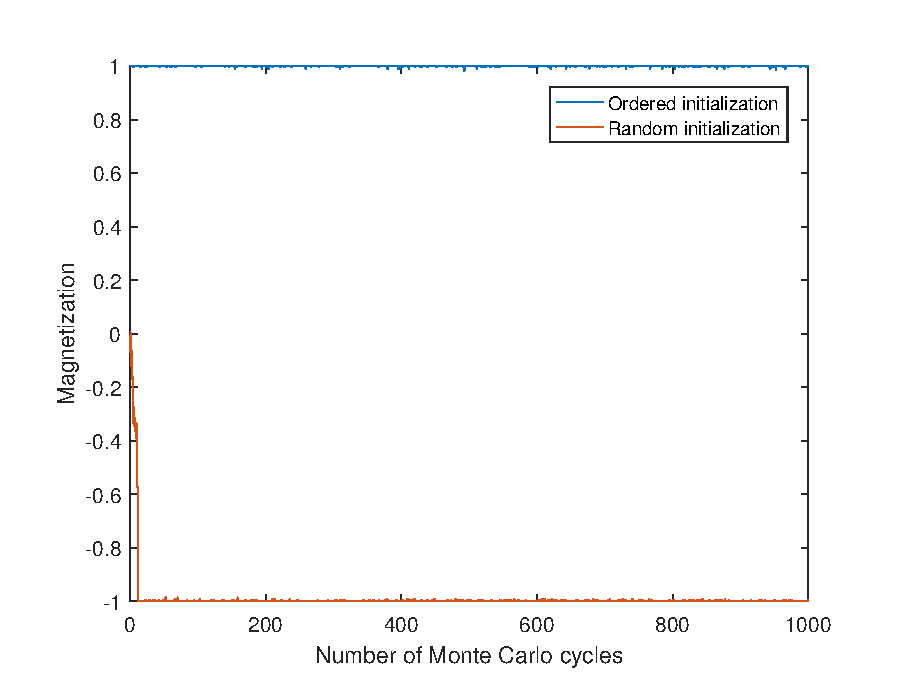
\includegraphics[width=0.8\textwidth]{Process_mag_lowT.eps}
	\caption{Magnetization as a function of the number of Monte Carlo cycles for $T=1.0$, $L=20$. }
\end{figure}
\end{frame}

\begin{frame}{Convergence and probability distribution}
\begin{figure}
	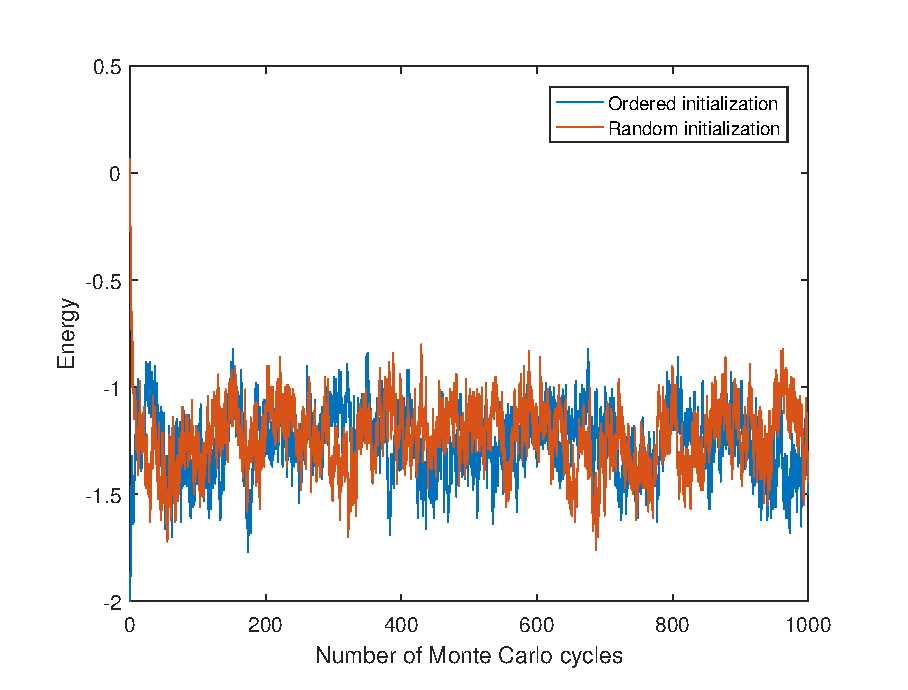
\includegraphics[width=0.8\textwidth]{Process_ene_highT.eps}
	\caption{Energy as a function of the number of Monte Carlo cycles for $T=2.4$, $L=20$. }
\end{figure}
\end{frame}

\begin{frame}{Convergence and probability distribution}
\begin{figure}
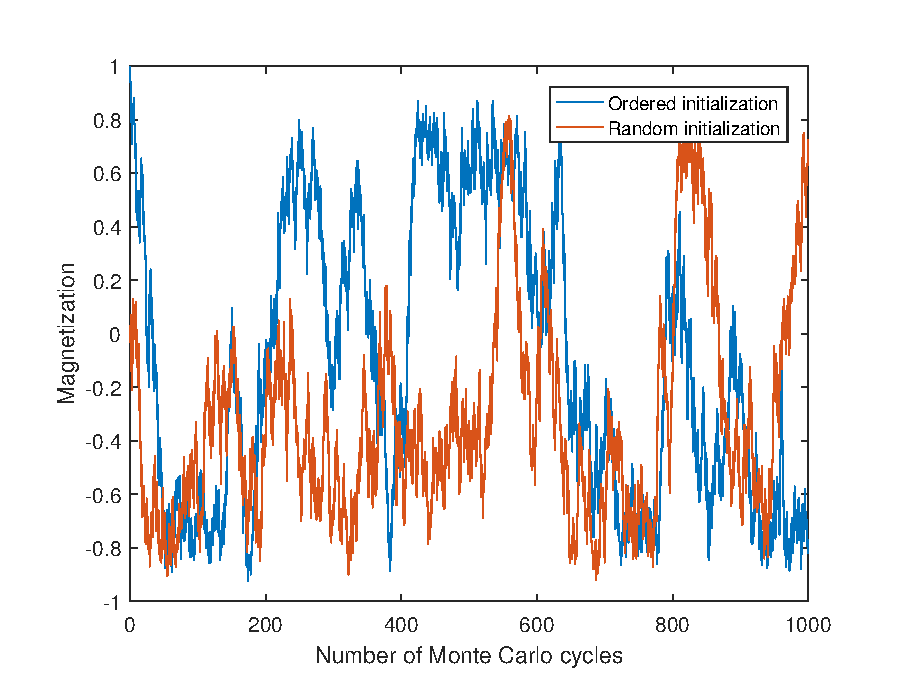
\includegraphics[width=0.8\textwidth]{Process_mag_highT.eps}
\caption{Magnetization as a function of the number of Monte Carlo cycles for $T=2.4$, $L=20$. }
\end{figure}
\end{frame}

\begin{frame}{Convergence and probability distribution}
\begin{figure}
	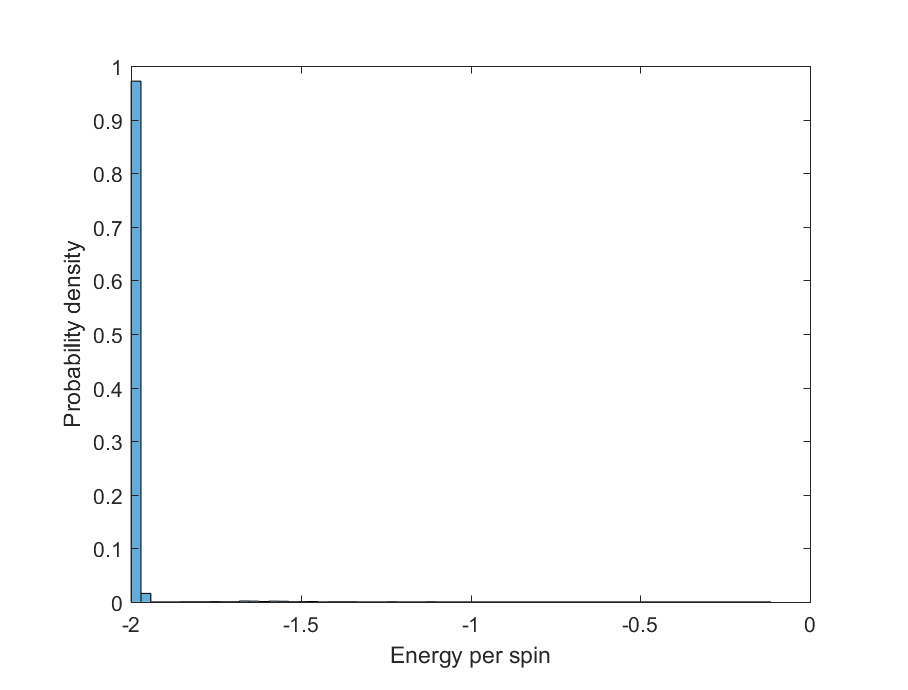
\includegraphics[width=0.8\textwidth]{Prob_ene_lowT.eps}
	\caption{Distribution of energy for $T=1.0$, $L=20$. }
\end{figure}
\end{frame}

\begin{frame}{Convergence and probability distribution}
\begin{figure}
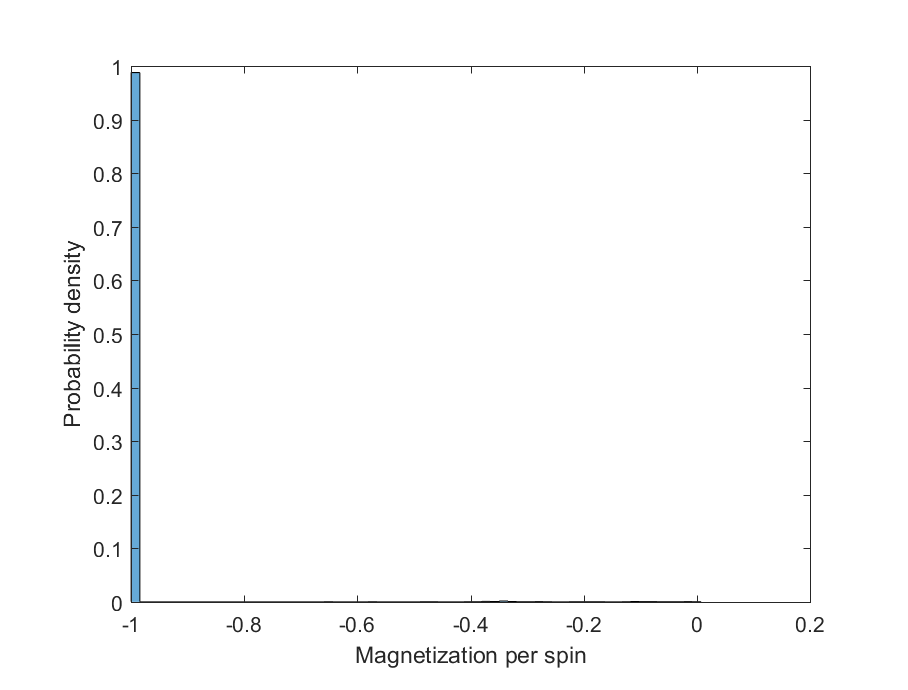
\includegraphics[width=0.8\textwidth]{Prob_mag_lowT.eps}
\caption{Distribution of magnetization for $T=1.0$, $L=20$. }
\end{figure}
\end{frame}

\begin{frame}{Convergence and probability distribution}
\begin{figure}
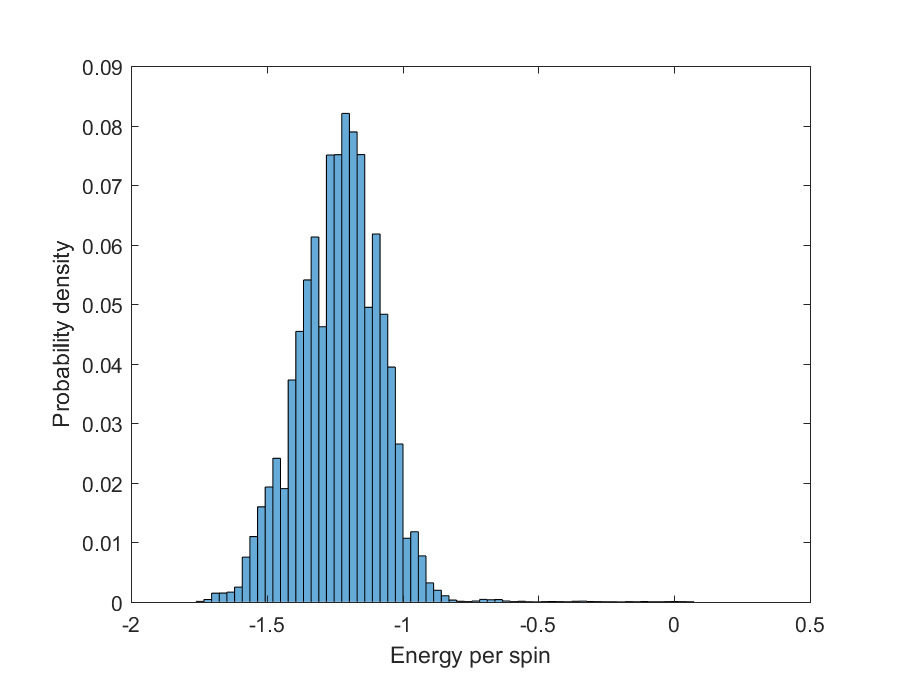
\includegraphics[width=0.8\textwidth]{Prob_ene_highT.eps}
\caption{Distribution of energy for $T=2.4$, $L=20$. }
\end{figure}
\end{frame}

\begin{frame}{Convergence and probability distribution}
\begin{figure}
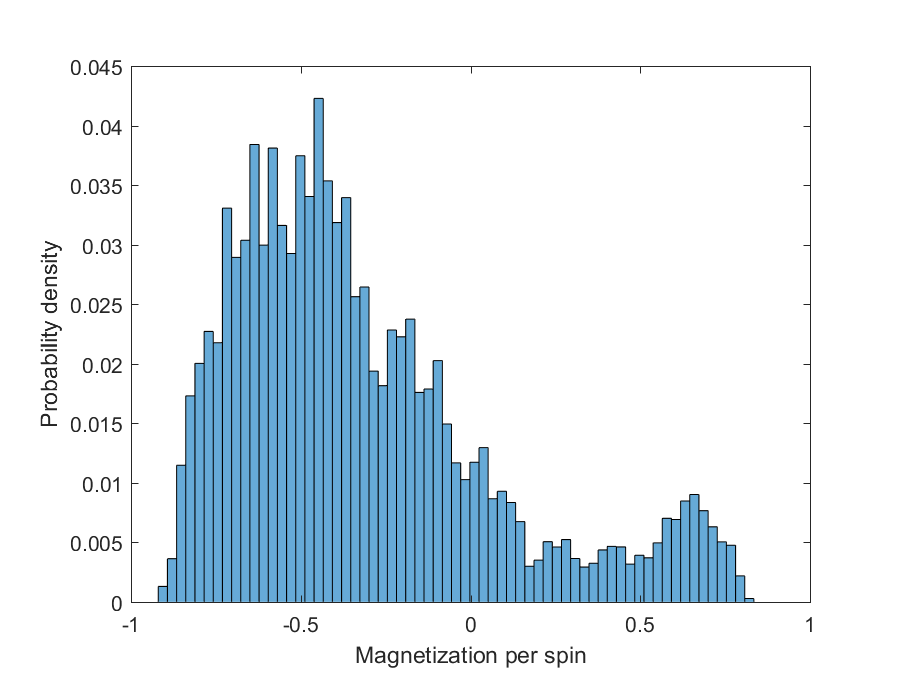
\includegraphics[width=0.8\textwidth]{Prob_mag_highT.eps}
\caption{Distribution of magnetization for $T=2.4$, $L=20$. }
\end{figure}
\end{frame}

\subsection{Phase transition}
\begin{frame}{Phase transition}
\begin{figure}
	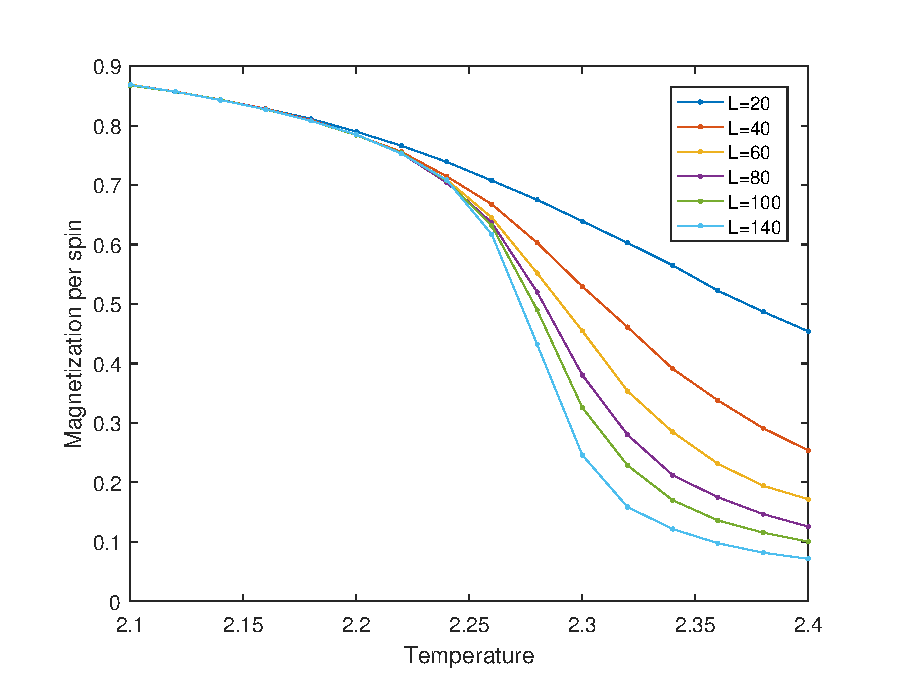
\includegraphics[width=0.8\textwidth]{Tran_mag.eps}
	\caption{Magnetization per spin as a function of temperature. Temperature step is 0.02 and the number of Monte Carlo cycles is $10^6$.  }
\end{figure}
\end{frame}

\begin{frame}{Phase transition}
\begin{figure}
	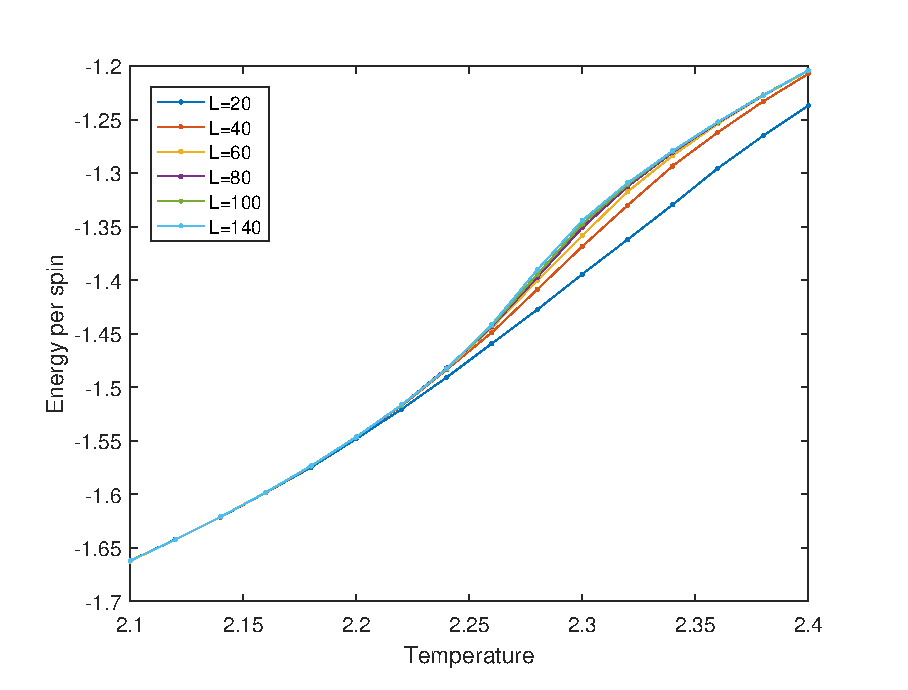
\includegraphics[width=0.8\textwidth]{Tran_ene.eps}
	\caption{Energy per spin as a function of temperature. Temperature step is 0.02 and the number of Monte Carlo cycles is $10^6$.  }
\end{figure}
\end{frame}

\begin{frame}{Phase transition}
\begin{figure}
	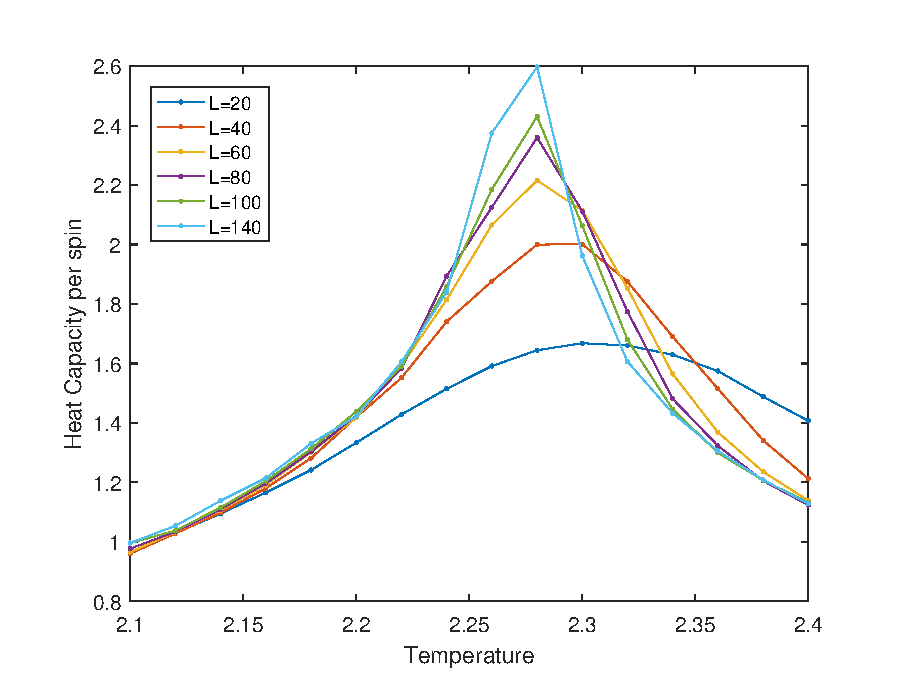
\includegraphics[width=0.8\textwidth]{Tran_Cv.eps}
	\caption{Heat capacity per spin as a function of temperature. Temperature step is 0.02 and the number of Monte Carlo cycles is $10^6$.  }
\end{figure}
\end{frame}

\begin{frame}{Phase transition}
\begin{figure}
	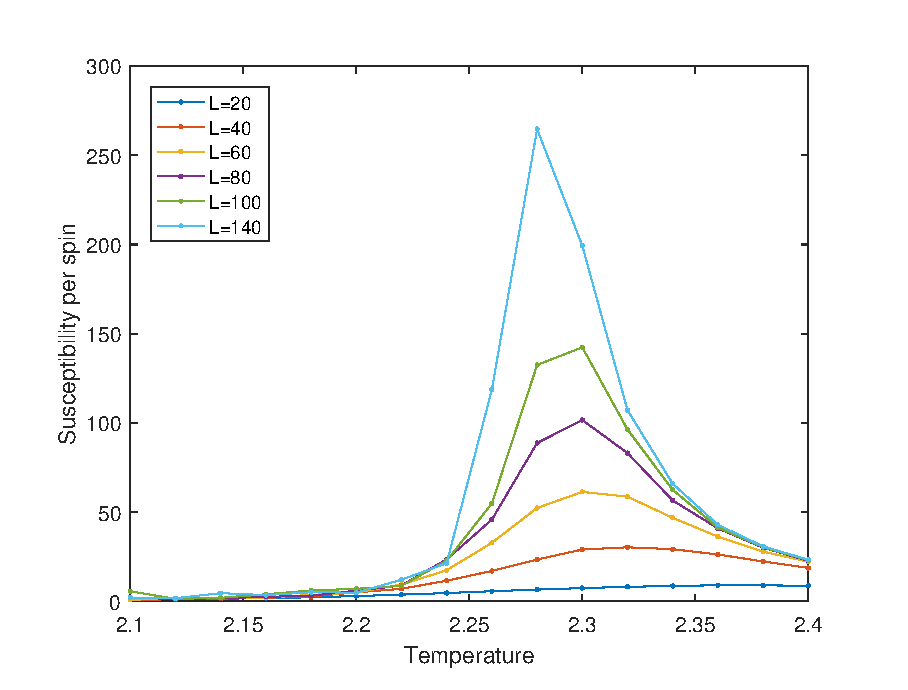
\includegraphics[width=0.8\textwidth]{Tran_sus.eps}
	\caption{Susceptibility per spin as a function of temperature. Temperature step is 0.02 and the number of Monte Carlo cycles is $10^6$.  }
\end{figure}
\end{frame}

\begin{frame}{Estimation of critical temperature}
\begin{itemize}
\item<1-> By the following equation 
\begin{equation}
T_C(L)-T_C(L=\infty) = aL^{-1/\nu}\,,
\label{eq:tc}
\end{equation}
where $a$ is a constant and $\nu=1$, 
we can estimate $T_C$ for an infinitely large system from the results with finite $L$. 
\item<2->
It is quite difficult to determine the critical temperature from previous figures 
because our resolution is not small enough. 
\item<3->
From the peaks of $\chi$ we estimate that $T_C(L=60)=2.3$ and $T_C(L=140)=2.28$. 
Then we obtain 
\begin{equation}
\left\{
\begin{array}{c}
a=2.1\,,  \\
T_C(L=\infty)=2.265\,.  \\
\end{array}
\right.
\end{equation}
\item<4-> Our estimation is close to the analytical result 2.269.
\end{itemize}
\end{frame}

\section{Conclusions}
\begin{frame}{Outline}
\tableofcontents[currentsection]
\end{frame}

\begin{frame}{Conclusions}
\begin{itemize}
	\item<1-> Our numerical results of $L=2$ case agrees well with the analytical values, 
	and calculations of $L=20$ case to confirm that the system converges fast to equilibrium in the simulation. 
	\item<2-> As expected the energy distribution centers around the mean value and a higher temperature leads to a broader distribution. 
	\item<3-> In phase transition, the behaviors of different physical quantities agree well with the analytical solution. 
	\item<4-> From the peak of susceptibility we estimate that the critical temperature for infinitely large lattice is 2.265, 
	which is close to the analytical value 2.269. 
	\item<5-> This work provides a powerful tool for the simulation of 2D Ising model, which can be extended to three-dimensional case. 
\end{itemize}
\end{frame}

\section*{Acknowledgment}
\begin{frame}{Acknowledgment}
	I am grateful for the sincere guidance from Prof. Morten Hjorth-Jensen. 
	\par
	Thanks for your attention! Any question? 
\end{frame}

\end{document}
